\chapter{Related Work}
\label{cha:related-work}

Because our approach combines work in various areas of distributed
systems debugging, from continuous record and replay, over
replay-driven fault navigation, debugging at different levels of
abstraction and full-on distributed debugging, we have sub-divided our
treaty of related work in this chapter into sections for each of those
domains.

\section{Record and Replay}
\label{sec:record-replay}

The need for consistent record and replay to debug certain kinds of
distributed applications is widely accepted. Approaches vary mainly in
how much they record, and subsequently how much of the system they can
simulate to eliminate behavioral disturbance.

\paragraph{Replay with Mocks}
\label{sec:replay-with-mocks}

Mocks are program entities designed to simulate the behavior of a real
entity. In system replay, mocks may be used to stand in for network
nodes. If enough information about the data sent by a particular node
has been recorded, there is no need to re-execute that node during
replay. Assuming the node works deterministically, a mock can return
the appropriate responses.

This approach is advantageous for nodes that are not under debugger
control. On those machines, package races on the network cannot be
rescheduled upon receive and behavior may still vary during
replay. Mocks avoid that problem, at the cost of greater recording
overhead at least in space, if not in time, for copying message
contents.

We have opted not to use mocks in this work, but other approaches use
mocks for some or all the nodes during a replay.

\paragraph{Deterministic Replay on the JVM with DejaVu}
\label{sec:dejavu}

\emph{DejaVu}~\cite{Konuru2000} is a record and replay framework for
distributed Java applications. It uses modified \acp{jvm} to execute
java applications and record their thread schedules as well as network
access. Thread and network schedules use implementations of Lamport
Clocks to establish event order.

The level of abstraction for network events in DejaVu is lower than in
this work, recording \ac{tcp} instead of \ac{http} events. While this
enables replay just as well, we argue that it is harder for a
programmer to review \ac{tcp} traffic and connect it to the program
domain than it is with \ac{http} events.

Contrary to this work, DejaVu supports both open and mixed world
record and replay. we note in \autoref{sec:distr-repl-reord} how the
same may be accomplished in my implementation.

\paragraph{Tracing and Simulation with iDNA}
\label{sec:idna}

\emph{iDNA}~\cite{Bhansali2006} is part of Microsoft-developed
framework for instruction-level tracing and replay of applications in
user-mode. The solution includes running instrumented programs atop a
runtime called \emph{Nirwana}, which provides hooks for iDNA to
register points of interest for tracing. The Nirwana runtime uses
dynamic binary translation to break a monitored process' instructions
into smaller instructions that are then instrumented and executed on
the host. The iDNA tracing component records traces via callbacks from
the Nirwana framework and, for replay, reads trace records and feeds
Nirwana desired instruction pointer and register values for
replay. The overhead is about one order of magnitude, which makes it
feasible to run IO-bound applications in tracing mode all the time,
which is also the scenario envisioned by the authors.

Due to its low level of recording, iDNA supports multi-threaded
applications, as well as applications that generate executable code at
runtime, such as \ac{jit}-compiled languages, but does not target networked
applications specifically. Similar to the present work, iDNA is aimed
at tracing continually on the live system, but the focus is on single
process applications rather than communicating processes or servers.

\paragraph{Reproducible Failures with ReCrash}
\label{sec:recrash}

\emph{ReCrash}~\cite{Artzi} is a framework to observe program execution in
Java and generate test-cases that reproduce observed errors. Similar
to this work, it can be applied to live systems. ReCrash does not try
to preserve enough information to replay an observed failure from the
beginning, but rather just keep enough information around to provide
an method entry point with arguments that trigger the crash.

To do this, ReCrash keeps a \emph{n}-deep \emph{shadow stack} during
execution with copies of the receivers and arguments. If a crash
occurs the stack is saved. In a second step, the shadow stack is
searched for the first call that reliably reproduces the exception.

The ability to reproduce crashes using this technique is limited by
the size of the shadow stack, as well as the copy depth of receiver
and arguments at each stage. Deeper stack and copying might be more
able to reproduce a crash, but imposes a larger overhead. The authors
offer a way out by only enabling monitoring after a crash occurred for
the first time, and only for methods on the stack at that point. Since
in this mode \emph{no} information has been saved about the execution,
the crash has to occur again, which might take a very long time for
rare exceptions.

For the class of problems that are related to causes that are not on
the same stack, like the concurrent update problem presented in this
thesis, ReCrash has only limited value.

\paragraph{Output-deterministic Replay with liblog}
\label{sec:liblog}

The \emph{liblog}~\cite{Geels2006Replay} tool for distributed C/C++
applications uses a {\tt libc} wrapper library to intercept system
calls and record events such as network communication, file access,
and \ac{ipc}.

The goal, as in this work, is to record sufficient information in the
live-system to replay execution at will for later debugging. The
authors decided against \emph{in-situ} replay, however, and use a
central console to download all logs and program checkpoints to
re-instantiate the program locally. Additionally, they record enough
information to replay each process independently of the others, which
imposes a higher tracing overhead.

Like DejaVu, and unlike this work, liblog records events at a very low
level. Most programs written for the Web, for example, do not use
socket programming directly, so the programmer will still have to
match the recorded network communication to the level of abstraction
in his code.

\section{Replay-driven Fault Navigation}
\label{sec:replay-driven-fault-1}

\paragraph{Test-driven Fault Navigation with Path Tools}
\label{sec:pathtools}

The \emph{Path Tools}~\cite{Perscheid} are a research project in
Squeak/Smalltalk and the basis for our prototype. Path Tools uses
re-executable entry points, mostly tests, to exercise code paths in a
project for analysis. These entry points need to execute
deterministically in order for the Path Tools' analysis to work
correctly.

In our work we have extended Path Tools and use it for re-execution
and analysis of distributed applications. Because Path Tools currently
need deterministic execution paths to work, this work offers an
approach to make network communication deterministic.

\section{Debugging at Different Levels of Abstraction}
\label{sec:debugg-at-diff-1}

\paragraph{Network Analysis and Debugging with Firebug}
\label{sec:firebug}

\emph{Firebug}\footnote{Mozilla Firebug:
  \url{http://getfirebug.com/}\\
  accessed June 20, 2012} is an open-source debugger and Web
application analysis tool for \emph{Firefox}\footnote{Mozilla Firefox:
  \url{http://www.mozilla.com/}\\
  accessed June 20, 2012}. It offers a JavaScript debugger with
breakpoints and a network pane to review \ac{xhr} requests made from
the JavaScript code of the web-page. Firebug includes the ability to
log network communication and set breakpoints on incoming and outgoing
connections, which enables developers to move from network to source
code, but not the other way around.

Firebug, like traditional debuggers, works synchronously on the code
and network communication of the current Web pages' JavaScript
process, and offers no integration with other services or debugger
instances. Also, while it is possible to break on network events and
move to the source code callback for a given event, there is no
further integration between the two~\cite{Barton2010}.

\paragraph{Message-oriented Debugging with Causeway}
\label{sec:causeway}

\emph{Causeway}\cite{Stanley2009} is a message-oriented debugger that
tries to unify the network request/response view with the message
send/receive view of the software. The authors' approach is to trace
program execution as well as network communication partners and
message contents, and present the captured information in a
post-mortem debugger. This debugger synchronizes the network and the
stack view so moving in one will update the other
(\cf{\autoref{fig:causeway}}), a behavior which has been the main
inspiration for how we show the two levels abstraction in our
prototype implementation.

In difference to this work, Causeway is strictly post-mortem. That
means it has to trace all required information, all the time, imposing
a very high overhead, a problem the authors mention themselves.

\begin{figure}[h]
  \centering
  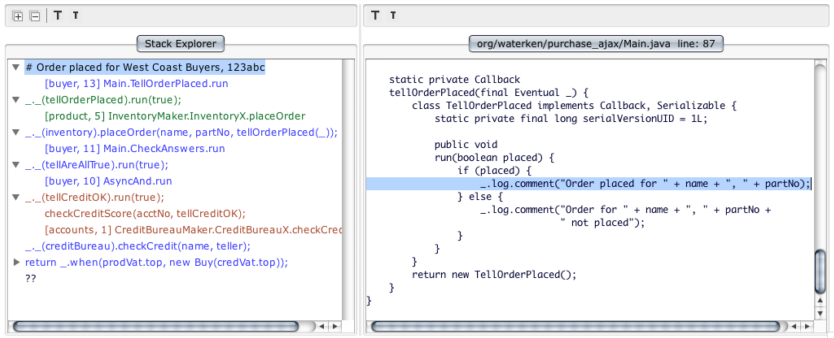
\includegraphics[width=0.7\linewidth]{causeway}
  \caption{Causeway Message Debugger}
  \label{fig:causeway}
\end{figure}

\section{Distributed Debugging}
\label{sec:distr-debugg}

Most debuggers work one thread at a time, and only for one process,
and offer the programmer a way to switch threads while debugging. Most
debuggers allow developers to stop all threads at once, however, this
disturb the execution order and lead to heisenbugs, since uniformly
starting and stopping multiple threads is not possible, even within a
single process. This equally applies to processes that are distributed
across a network. However, some runtimes, such as the \ac{jvm} or the
\ac{clr}, but also distributed systems middleware, such as
\textsc{corba}, still allow developers to stop and inspect processes
across a network.

\paragraph{Virtual Machine Interfaces on JVM and CLR}
\label{sec:java}

Both the \ac{jvm} and the \ac{clr} offer debugging facilities to
connect symbolic debuggers to remote processes. These facilities, in
case of the \ac{jvm} using a custom \ac{jvmti}\footnote{\textsc{jvm}
  Tool Interface Version 1.0\\
  \url{http://docs.oracle.com/javase/1.5.0/docs/guide/jvmti/jvmti.html}\\
  accessed July 31, 2012} and in case of the \ac{clr} built on the
\ac{com} standard~\cite{Strein2005}, abstract from the network to
offer the same debugging experience across a network as for local
processes. Debugging multiple processes from the same \ac{vm} is
possible with these approaches. Additionally, both of these \acp{vm}
are built to support different languages, so debugging across
languages is possible, too. However, we know of no debugging tool for
either \ac{vm} that supports different languages.

Compared to this work, these debugging interfaces have two
shortcomings: first, to inspect a remote process that process has to
be stopped by the debugger. It is undesirable for a deployed system to
stop providing its service because a debugger is connected to
it. Second, these debugging facilities only provide a view on the
program, and do not track network communication between processes, so
it is still difficult to get a global view of the distributed system.

\paragraph{Debugging Distributed Objects with CORBA and SOAP}
\label{sec:corba}

As a logical extension of object oriented programming into the realm
of distributed systems, middleware layers, such as
CORBA~\cite{Yang1996} and SOAP~\cite{Walsh2002}, have evolved. They
allow developers of distributed systems to specify object interfaces
for publishing and accessing distributed services in an
interchangeable format. Developers can program against these
interfaces as if the distributed system were running in a single
process, while the middleware takes care of communication. However,
much of the development time complexity hiding provided by middleware
is lost when debugging, because developers cannot step into message
sends that are converted to network communication by the
middleware. Recently, effort has been expended to enable symbolic
debuggers to overcome this restriction and step across
servers~\cite{Mega,Kaler2007} when debugging on top of such
middleware.

Such debuggers for middleware systems, like the middleware systems
themselves, try to abstract from the network. Approaches at stepping
across servers are extensions to symbolic debuggers that are meant to
allow developers to inspect objects in distributed system as if they
were locally available. In contrast to this work, these debuggers
target systems that are fully under developer control and can be
stopped at will for inspection. Like traditional symbolic debuggers,
they ignore Heisenbugs caused by the debugging process and are not
well suited to debug non-deterministic failures.

%%% Local Variables: 
%%% mode: latex
%%% TeX-master: "thesis"
%%% End: 
